\section{Experimental Evaluation}
\label{sec:experiments}

\subsection{Experimental Protocol}

\paragraph{Dataset} 
\label{sec:dataset}

The proposed training methods are evaluated on the PASCAL
VOC 2012 segmentation benchmark \citep{everingham2014pascal},
consisting of 20 foreground object classes and one background
class. The performance is measured in terms of pixel
intersection-over-union (IOU) averaged across the 21 classes. The
original PASCAL VOC 2012 dataset contains $1464$ (\textsl{train}),
$1449$ (\textsl{val}), and $1456$ (\textsl{test}) images for training,
validation, and test, respectively. In some experiments we also use
the extra annotations provided by \citet{hariharan2011semantic},
resulting in augmented sets of $10,582$ (\textsl{train\_aug}) and
$12,031$ (\textsl{trainval\_aug}) images. We have also experimented
with the abundant annotations provided by the MS-COCO 2014 dataset
\citep{lin2014microsoft}, which contains $123,287$ images in its
\textsl{trainval} set. The MS-COCO 2014 dataset has $80$ foreground
object classes and one background class.

Evaluation of our proposed methods is primarily conducted on the
PASCAL VOC 2012 \textsl{val} set but we also report results of selected
method variants submitted to the official PASCAL VOC 2012 server, which
evaluates results on the \textsl{test} set (whose annotations are not
released).

\paragraph{Training}

We employ our proposed training methods to learn the DCNN component of
the DeepLab-CRF model of \citet{chen2014semantic}. We start with the
Imagenet pretrained VGG-16 network of \citet{simonyan2014very},
modified as described in \citet{chen2014semantic}. In SGD training, we
use a mini-batch of 20 images and initial learning rate of $0.001$
($0.01$ for the final classifier layer), multiplying the learning rate
by 0.1 after a fixed number of iterations. We use momentum of $0.9$
and a weight decay of $0.0005$. Fine-tuning our network on PASCAL VOC
2012 takes about 12 hours on a NVIDIA Tesla K40 GPU. Our
implementation is based on the publicly available Caffe software
\citep{jia2014caffe}.

Similarly to \citet{chen2014semantic}, we decouple the DCNN and Dense
CRF training stages and learn the CRF parameters by cross validation
so as to maximize IOU segmentation accuracy in a held-out set of 100
Pascal \textsl{val} fully-annotated images. We use 10 mean-field
iterations for Dense CRF inference \citep{krahenbuhl2011efficient}.

\paragraph{Weak annotations}

In order to simulate the situations where only weak annotations are
available and to have fair comparisons (e.g., use the same images for
all settings), we generate the weak annotations from the pixel-level
annotations. The image-level labels are easily generated by
summarizing the pixel-level annotations, while the bounding box
annotations are produced by drawing rectangles tightly containing each
object instance (PASCAL VOC 2012 also provides instance-level
annotations) in the dataset.

\subsection{Model Training Using Fully Annotated Images}
\label{sec:test_pixel}

The performance of the DeepLab-CRF model trained with strong
pixel-level annotations sets a target upper bound which we try to
reach with the proposed algorithms for weakly- or semi-supervised
training. In reproducing the results of \citep{chen2014semantic} on
PASCAL VOC 2012 \textsl{val}, we have achieved a
\textsl{DeepLab-CRF(Strong)} IOU score of \textbf{63.93}\% (they
report a score of 63.74 in their Table~1a).

%% \begin{table}
%%   \centering
%%   \caption{{\bf{Pixel Annotations.}} Performance on the PASCAL VOC 2012 `val' set. First column, and second column show the number of strongly labeled images from PASCAL and MS-COCO. }
%%   \begin{tabular}{| c | c | c | c |}
%%     \hline
%%     \# PASCAL & \# MS-COCO & DeepLab & DeepLab-CRF \\
%%     \hline
%%     10,582 &   0     & 59.85 & 63.93  \\
%%     \hline
%%     10,582 & 123,287 & 64.51 & 67.98 \\
%%     \hline
%%     \end{tabular}
%%   \label{tb:pixel_annot}
%% \end{table}

\subsection{Model Training Using Bounding Box Weak Annotations}
\label{sec:test_bbox}

In this experiment we train the DeepLab-CRF model using the PASCAL VOC
2012 bounding box annotations, generated as described in
\secref{sec:dataset} above. We estimate the training set segmentations
in a pre-processing step using the \textsl{Bbox-Baseline} and
\textsl{Bbox-Seg} methods described in \secref{sec:train_bbox}.

We assume that we also have access to 100 fully-annotated PASCAL VOC
2012 \textsl{val} images which we have used to cross-validate the
value of the single \textsl{Bbox-Seg} parameter $\alpha$ (percentage
of the center bounding box area constrained to be foreground). We
varied $\alpha$ from 20\% to 80\%, as shown in
\tabref{tb:bbox_erosion}. We found that using $\alpha = 20\%$
maximizes the accuracy in terms of IOU in recovering the ground truth
foreground from the bounding box.

\begin{table}
  \centering
  \caption{\textsl{Bbox-Seg} parameter cross-validation.}
  \begin{tabular}{c | c c c c}
    \alpha (\%)    &  80   &  60   &  40   &  20   \\
    \hline
    Pixel IOU (\%) & 65.6  & 68.8  & 71.8  & {\bf 72.6}
    \end{tabular}
  \label{tb:bbox_erosion}
\end{table}

The PASCAL VOC 2012 \textsl{val} performance achieved after training
the DeepLab-CRF model on the segmentations obtained by the
\textsl{Bbox-Baseline} and \textsl{Bbox-Seg} is reported in
\tabref{tb:bbox_annot}. We see that \textsl{Bbox-Seg} improves over
\textsl{Bbox-Baseline} by nearly 6\% but still lags by 5.5\% compared
to training with the strong pixel-level annotation.

\begin{table}
  \centering
  \caption{DeepLab-CRF VOC 2012 \textsl{val} performance using
    bounding box weak annotations \vs strong annotation in training.}
  \scalebox{0.9}{
  \begin{tabular}{c | c || c}
    Bbox-Baseline & Bbox-Seg & Strong \\
    \hline
    52.52         & 58.45    & 63.93
  \end{tabular}
  }
  \label{tb:bbox_annot}
\end{table}

%% \begin{table}
%%   \centering
%%   \caption{{\bf Bounding Box Annotations.} Performance on the PASCAL VOC 2012 `val' set. DeepLab and DeeLab-CRF are trained with the segmentation generated by Bbox-Baseline or Bbox-DenseCRF.}
%%   \begin{tabular}{| l | c | c |}
%%     \hline
%%      & DeepLab & DeepLab-CRF \\
%%     \hline
%%     Bbox-Baseline & 47.72 & 52.52 \\ 
%%     \hline
%%     Bbox-DenseCRF & 53.68 & 58.45 \\
%%     \hline
%%     \end{tabular}
%%   \label{tb:bbox_annot}
%% \end{table}

\subsection{Model Training Using Weak Image-Level Labels}
\label{sec:test_image}

We proceed with evaluating our proposed methods in training the
DeepLab-CRF model using just image-level weak PASCAL VOC 2012
annotations, generated as described in \secref{sec:dataset} above. We
report the \textsl{val} performance of our two weakly-supervised EM
variants described in \secref{sec:train_weak}. In the
\textsl{EM-Fixed} variant we use $c_f = 6$ and $c_b = 5$ as fixed
foreground and background biases. We found the results to be quite
sensitive to the difference $c_f-c_b$ but not very sensitive to their
absolute values. In the adaptive \textsl{EM-Adapt} variant we
constrain at least 40\% of the image area to be assigned to background
and at least 20\% of the image area to be assigned to foreground (as
specified by the weak label set). 

The PASCAL VOC 2012 \textsl{val} performance achieved after training
the DeepLab-CRF model with this weakly-supervised EM algorithm are
reported in \tabref{tb:weak_annot}. This table also contains results
obtained by the previous MIL-based methods \textsl{MIL1}
\citep{pathak2014fully} and \textsl{MIL2}, \textsl{MIL2-ILP}
\citep{pinheiro2014weakly}. Note that the numbers are not directly
comparable because \citet{pathak2014fully} evaluates on the VOC 2011
\textsl{val} and \citet{pinheiro2014weakly} train the parameters of
their CNN models on the Imagenet dataset. 

We observe that \textsl{EM-Fixed} performs poorly on this challenging
task, at the same level as the previous \textsl{MIL1} and \textsl{MIL2}
methods. Similarly to them, we observed that the \textsl{EM-Fixed}
model had particularly difficulty in balancing the scores of the
foreground and background classes, often producing all-background
segmentations. The \textsl{MIL2-ILP} method partially alleviates this
problem by departing from the pure MIL formulation, also incorporating
image-level classification scores during training. Our
\textsl{EM-Adapt} method performed considerably better by explicitly
enforcing both background and foreground labels to emerge in the
estimation process. However, its performance at 38.2\% significantly
lags the target 63.93\% goal of the strongly-supervised model trained
on pixel-level annotations.

\begin{table}
  \centering
  \caption{DeepLab-CRF VOC 2012 \textsl{val} performance using
    image-level weak annotations in training compared to previous methods.}
  \scalebox{0.9}{
  \begin{tabular}{c | c | c || c | c}
    MIL1  & MIL2 & MIL2-ILP & EM-Fixed & EM-Adapt \\
    \hline
    20.46 & 17.8 & 32.6     & 20.77    & 38.2
  \end{tabular}
  }
  \label{tb:weak_annot}
\end{table}


%% \begin{table}
%%   \centering
%%   \caption{{\bf Comparison with state-of-art methods on val set.}}
%%   \begin{tabular}{l|c}
%%     {\bf Method} & pixel IOU (\%) \\
%%     \hline \hline
%%     Idiap-base   & 17.8 \\
%%     DeepLab-Weak & 20.3 \\
%%     \hline \hline
%%     Idiap-base+ILP  & 32.6 \\
%%     DeepLab-Adaweak & 34.2 \\
%%     \hline \hline
%%     Idiap-base+ILP+sppxl & 36.6 \\
%%     DeepLab-CRF-Adaweak  & 38.2 \\
%%     \hline \hline
%%     Idiap-base+ILP+seg       & 42.0 \\
%%     DeepLab-CRF-StrongWeak   & 61.9 \\
%%   \end{tabular}
%%   \label{tab:weak_state_of_art_val}
%% \end{table}


\subsection{Semi-Supervised Model Training Using Both Fully and Weakly Annotated Images}
\label{sec:test_semi}

We next examine to what extent weak image-level annotations can
complement strong pixel-level annotations in training the DeepLab-CRF
model, using the semi-supervised learning methods of
\secref{sec:train_semi}. In this experiment we employ the strong
annotations of a subset of PASCAL VOC 2012 \textsl{train} set and
use just the weak image-level labels from another non-overlapping
subset of the \textsl{train\_aug} set. We perform segmentation
inference for the images that only have image-level labels by means of
\textsl{EM-Fixed}. In \tabref{tab:strong_weak_annot} we report the 
results obtained by varying the sizes of the strong and weak
annotation sets, also including for comparison the results of pure
weakly-supervised and strongly-supervised learning.

We observe that including even a few hundreds of strongly annotated
images in the semi-supervised setting significantly improves the 
performance compared to the pure weakly-supervised baseline. We also
observe that using just 1,464 strongly annotated images (13.8\% of the
\textsl{train\_aug} set) along with the remaining weakly annotated
images suffices to reach performance 61.90\%, only 2\% lower than the
pure strongly-supervised target. Note that only using the 1,464
strongly annotated images and no weakly annotated images performs
significantly worse at 57.62\%, demonstrating the significant benefits
of the semi-supervised setting.

\begin{table}[t]
  \centering
  \caption{DeepLab-CRF VOC 2012 \textsl{val} performance using
    both strong pixel-level and weak image-level annotations.}
  \scalebox{0.8}{
  \begin{tabular}{|c|c|c|}
    \hline
    Strong & Weak & DeepLab-CRF\\
    \hline
    0        &  10,582 & 20.77 (\textsl{EM-Fixed}) \\
    0        &  10,582 & 38.23 (\textsl{EM-Adapt}) \\
    \hline\hline
    200      &  10,382 & 47.57   \\
    500      &  10,082 & 56.89   \\
    750      &  9,832  & 58.82   \\
    1,000    &  9,582  & 60.48   \\
    \hline
    1,464    &  0      & 57.62   \\
    1,464    &  5,000  & 60.48   \\
    1,464    &  9,118  & 61.90   \\
    \hline\hline
    10,582   &  0      & 63.93 (\textsl{Strong}) \\
    \hline
  \end{tabular}  
  }
  \label{tab:strong_weak_annot}
\end{table}


%% \begin{table}[t]
%%   \centering
%%   \caption{{\bf Pixel+Image Annotations.} }
%%   \scalebox{0.8}{
%%   %\addtolength{\tabcolsep}{-2.0pt}
%%   \begin{tabular}{|c|c|c|c|}
%%     \hline
%%     {\bf Weak} & {\bf Strong} & \multirow{2}{*}{DeepLab} & \multirow{2}{*}{DeepLab-CRF}\\
%%     \cline{1-2}
%%     \# PASCAL & \# PASCAL & & \\
%%     \hline
%%     10,582   &    0    & 20.25  & 20.77   \\
%%     \hline
%%     10,582   &    0    & 34.22* & 38.23*  \\
%%     \hline
%%     10,382   &  200    & 44.05  & 47.57   \\
%%     \hline
%%     10,082   &  500    & 52.52  & 56.89   \\
%%     \hline
%%     9,832    &  750    & 55.04  & 58.82   \\
%%     \hline
%%     9,582    &  1,000  & 56.79  & 60.48   \\
%%     \hline
%%       0      &  1,464  & 54.77  & 57.62   \\
%%     \hline
%%     5,000    &  1,464  & 57.02  & 60.48   \\
%%     \hline
%%     9,118    &  1,464  & {\bf 58.30}  & {\bf 61.90}   \\
%%     \hline
%%   \end{tabular}  
%%   }
%%   \label{tab:strong_weak_annot}
%% \end{table}


\subsection{Exploiting Annotations Across Datasets}
\label{sec:cross_dataset}

Finally, we discuss how we can exploit annotations across different
datasets potentially having different label spaces, also allowing for
the possibility annotations to be in part weak and in part strong. We
have conducted experiments leveraging the 81-label MS COCO dataset as
an additional source of data in learning the DeepLab model for the
21-label Pascal VOC 2012 segmentation task. We have considered the
following scenarios:
\begin{enumerate}
\item Pre-train DeepLab on MS-COCO, then replace the top-level
  classifiers weights and fine-tune on Pascal VOC 2012, using strong
  labels in both datasets.
\item Jointly train DeepLab on MS-COCO and Pascal VOC 2012 sharing
  the top-level classifier weights for the common classes, using
  strong labels in both datasets.
\item Jointly train DeepLab on MS-COCO and Pascal VOC 2012 sharing
  the top-level classifier weights for the common classes, using a
  combination of strong and weak labels.
\end{enumerate}

We then exploited the rich annotations provided by MS-COCO
dataset: the models are fine-tuned on PASCAL VOC after fine-tuning on
MS-COCO. As shown in Tab.~\ref{tb:pixel_annot}, training the models
with a large amount of full annotations further improves both DeepLab
and DeepLab-CRF by about $4\%$ on the validation set.

\subsection{Qualitative results} 
\label{sec:test_qualitative}

We provide visual comparisons between our proposed models in
Fig.~\ref{fig:ValResults}. The results with exploiting only weak
labels (DeepLab-CRF-Adaweak) are relatively noisy compared to other
methods. Training the model with only Bbox-Baseline
(DeepLab-CRF-Bbox-Baseline) gives very crude results, while the
results from the model (DeepLab-CRF-Bbox-DenseCRF) trained with the
estimated segmentation by Bbox-DenseCRF are visually better. Jointly
training the model (DeepLab-CRF-StrongWeak) with a small number of
full annotations and many weak annotations can further improve the
results qualitatively. The results from the model (DeepLab-CRF-COCO)
trained with both strong annotations from PASCAL and MS-COCO are the
best.


\subsection{Evaluation on Test set and Comparison with State-of-Art}

After setting the model choices on the validation set, we evaluate our
variant models on the PASCAL VOC 2012 official test set. The results
from our models along with other state-of-art models are listed in
Tab.~\ref{tab:voc2012}. 

Given only weak labels, our DeepLab-CRF-Adaweak is better than Idiap-base+ILP+sppxl \citep{pinheiro2014weakly}. 

In the context of bounding box annotations, training our models with the segmentation inferred by Bbox-DenseCRF is $6.2\%$ better than with crude segmentation from Bbox-Baseline. Note that our DeepLab-CRF-Bbox-DenseCRF is comparable to other fully supervised models, such as Hypercolumn-SDS \citep{hariharan2014hypercolumns}.

Our DeepLab-CRF-StrongWeak takes use of both strong and weak annotations during training. DeepLab-CRF-StrongWeak1 exploits 1464 fully annotated images (PASCAL train set), while DeepLab-CRF-StrongWeak2 uses 2913 fully annotated images (PASCAL trainval set). DeepLab-CRF-StrongWeak1 has better performance (absolute $22.9\%$ improvement) than Idap-base+ILP+reg, showing that directly leveraging fully annotated images during training is better than resorting to some region proposal algorithms. Note that DeepLab-CRF-StrongWeak2 delivers the same performance as DeepLab-CRF \citep{chen2014semantic}, which is trained with about 12K fully annotated images. Furthermore, our DeepLab-CRF-StrongWeak2 outperforms many fully supervised models, including TTI-Zoomout-16 \citep{mostajabi2014feedforward}, FCN-8s \citep{long2014fully}, and MSRA-CFM \citep{dai2014convolutional}.

Last, our DeepLab-CRF-COCO is fine-tuned on MS-COCO dataset before fine-tuning on PASCAL augmented trainval set. This model sets a new state-of-art result.


\begin{table}[t]
  \centering
  \caption{{\bf Pixel+Image Annotations with MS-COCO.} }
  \scalebox{0.77}{
  %\addtolength{\tabcolsep}{-2.0pt}
  \begin{tabular}{|c|c|c|c|c|}
    \hline
    {\bf Weak} & \multicolumn{2}{c|}{\bf Strong} & \multirow{2}{*}{DeepLab} & \multirow{2}{*}{DeepLab-CRF}\\
    \cline{1-3}
    \# MS-COCO & \# PASCAL & \# MS-COCO & & \\
    \hline
      0       & 10,582 & 0       & 59.85 & 63.93 \\
    \hline
      123,287 & 10,582 & 0       & 60.41 & 64.44 \\
    \hline
      0       & 10,582 & 5,000   & 61.34 & 64.91 \\
    \hline
      118,287 & 10,582 & 5,000   & ?     &  ?    \\
    \hline    
      0       & 10,582 & 123,287 & 64.51 & 67.98 \\
    \hline
  \end{tabular}  
  }
  \label{tab:strong_weak_annot_coco}
\end{table}


\begin{figure*}[!htbp]
  \centering
  %\vspace{-1.cm}
  \scalebox{0.82} {
  \begin{tabular}{c c c c c c}
    %\addtolength{\tabcolsep}{-6.5pt}
    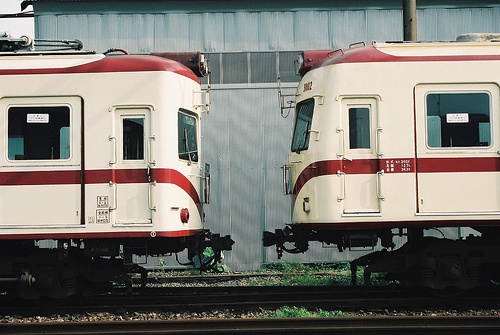
\includegraphics[height=0.11\linewidth]{fig/val_crf_vis/img/2007_000042.jpg} &
    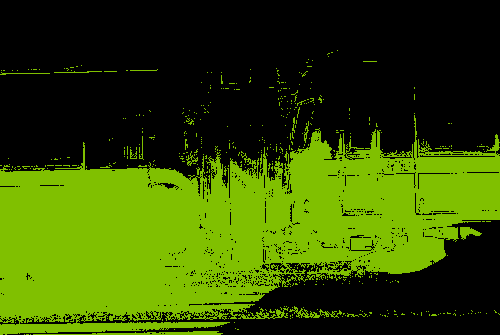
\includegraphics[height=0.11\linewidth]{fig/val_crf_vis/adaweak/2007_000042.png} &
    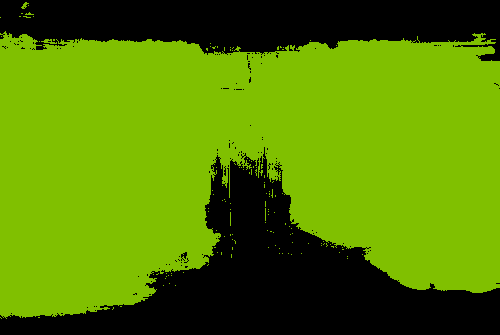
\includegraphics[height=0.11\linewidth]{fig/val_crf_vis/bbox/2007_000042.png} &
    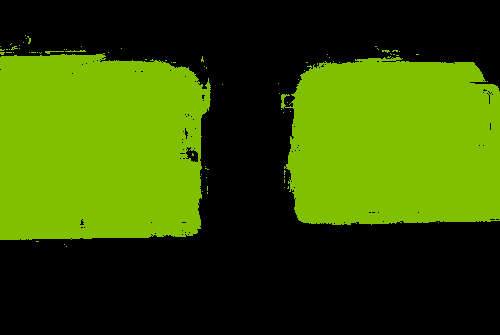
\includegraphics[height=0.11\linewidth]{fig/val_crf_vis/bbox_crf/2007_000042.png} &
    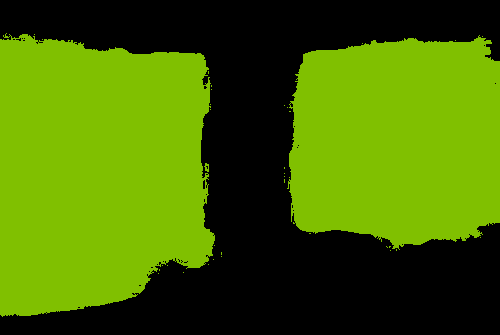
\includegraphics[height=0.11\linewidth]{fig/val_crf_vis/strongweak/2007_000042.png} &
    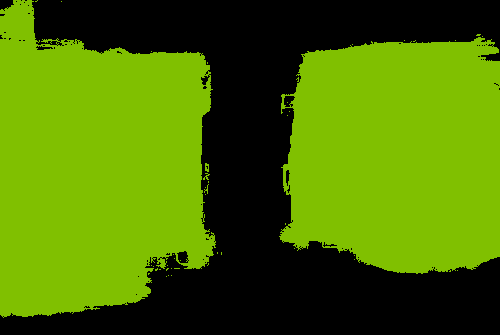
\includegraphics[height=0.11\linewidth]{fig/val_crf_vis/cocomix/2007_000042.png} \\
    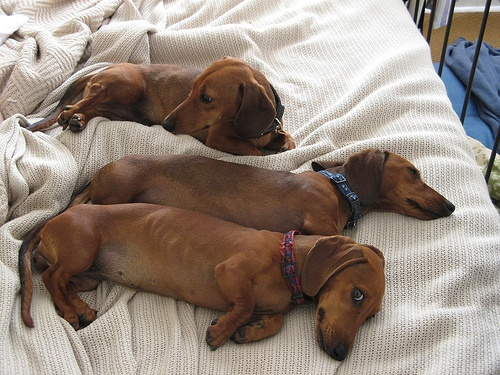
\includegraphics[height=0.122\linewidth]{fig/val_crf_vis/img/2007_002852.jpg} &
    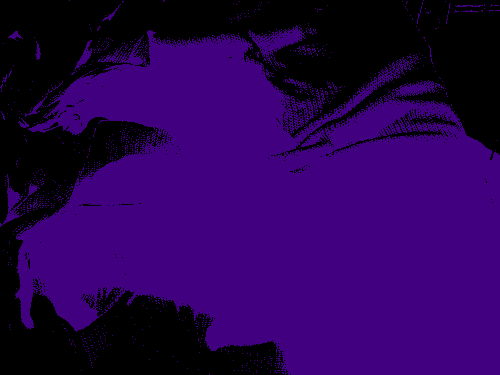
\includegraphics[height=0.122\linewidth]{fig/val_crf_vis/adaweak/2007_002852.png} &
    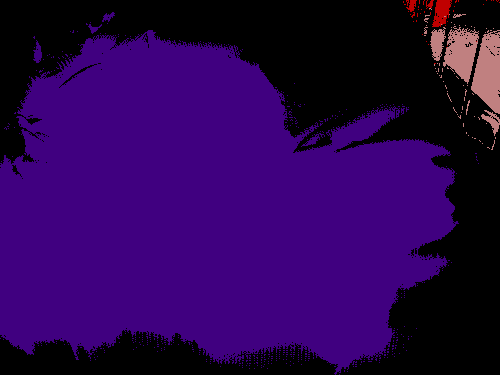
\includegraphics[height=0.122\linewidth]{fig/val_crf_vis/bbox/2007_002852.png} &
    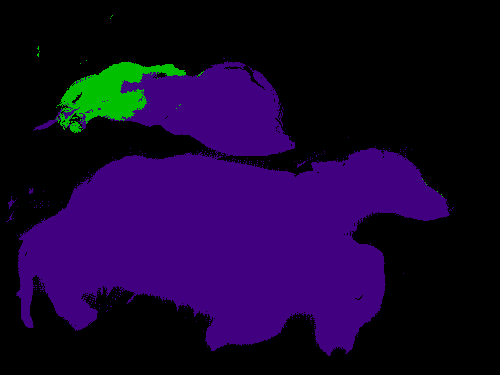
\includegraphics[height=0.122\linewidth]{fig/val_crf_vis/bbox_crf/2007_002852.png} &
    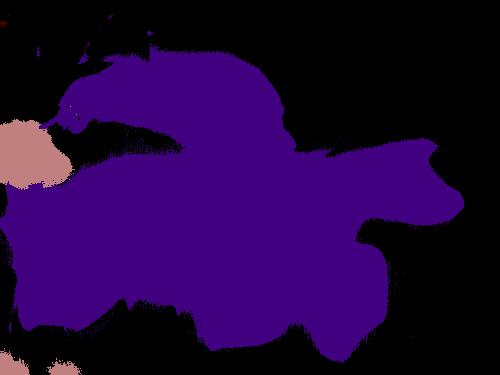
\includegraphics[height=0.122\linewidth]{fig/val_crf_vis/strongweak/2007_002852.png} &
    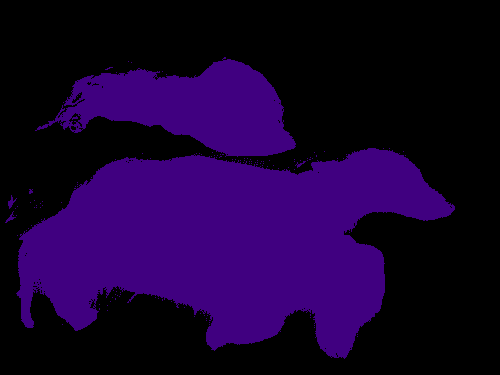
\includegraphics[height=0.122\linewidth]{fig/val_crf_vis/cocomix/2007_002852.png} \\
    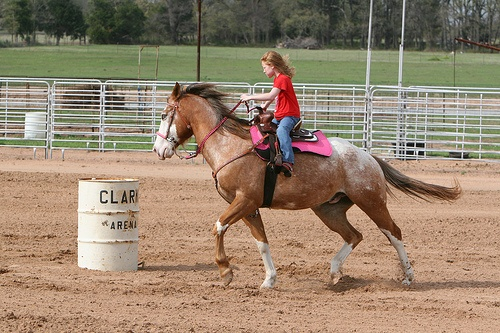
\includegraphics[height=0.11\linewidth]{fig/val_crf_vis/img/2007_003022.jpg} &
    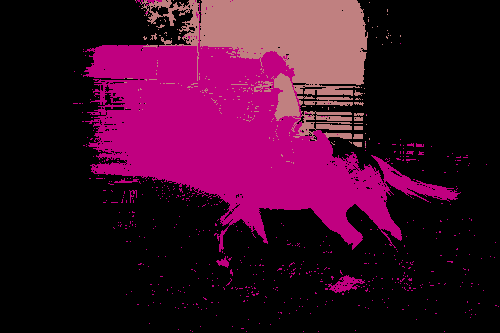
\includegraphics[height=0.11\linewidth]{fig/val_crf_vis/adaweak/2007_003022.png} &
    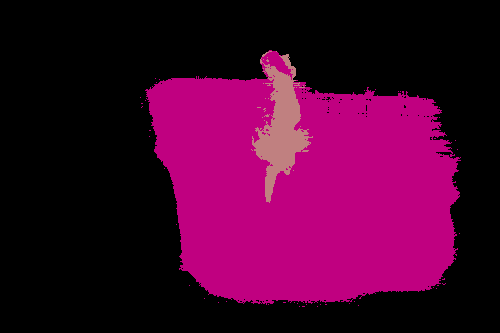
\includegraphics[height=0.11\linewidth]{fig/val_crf_vis/bbox/2007_003022.png} &
    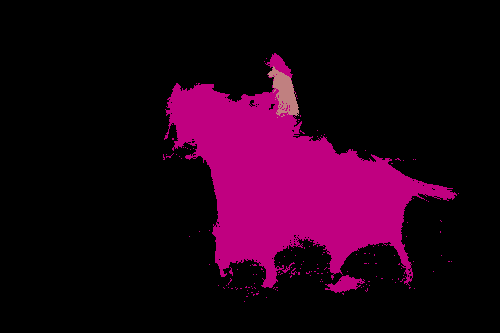
\includegraphics[height=0.11\linewidth]{fig/val_crf_vis/bbox_crf/2007_003022.png} &
    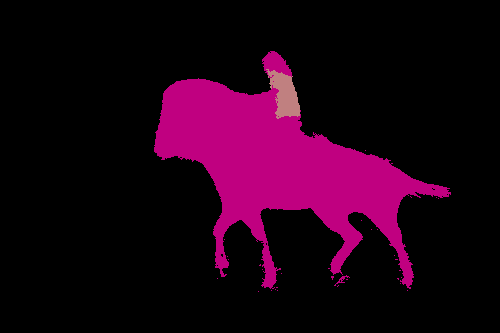
\includegraphics[height=0.11\linewidth]{fig/val_crf_vis/strongweak/2007_003022.png} &
    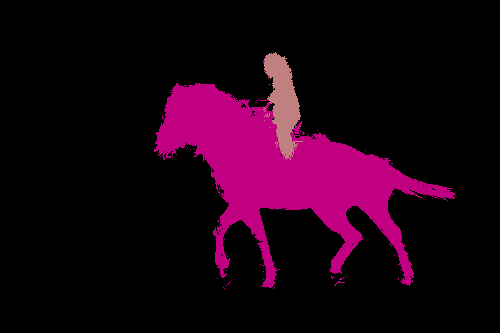
\includegraphics[height=0.11\linewidth]{fig/val_crf_vis/cocomix/2007_003022.png} \\
    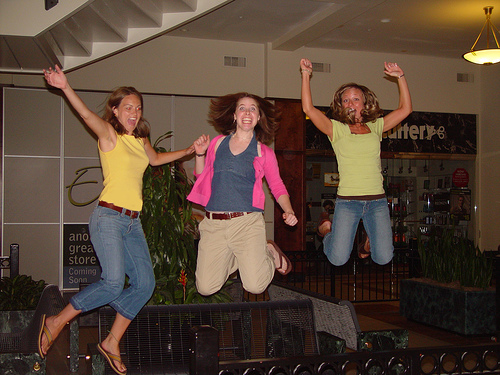
\includegraphics[height=0.123\linewidth]{fig/val_crf_vis/img/2008_003546.jpg} &
    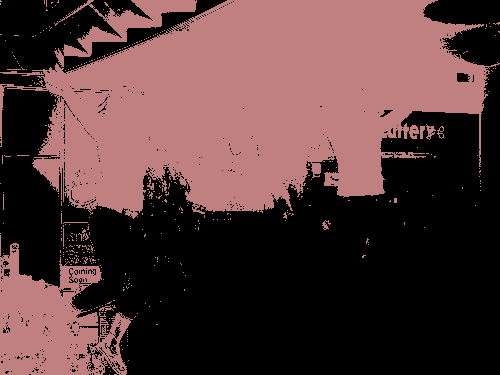
\includegraphics[height=0.123\linewidth]{fig/val_crf_vis/adaweak/2008_003546.png} &
    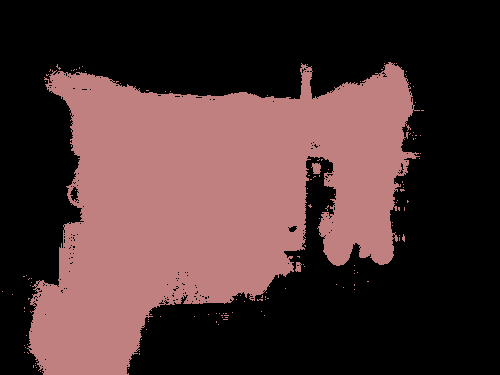
\includegraphics[height=0.123\linewidth]{fig/val_crf_vis/bbox/2008_003546.png} &
    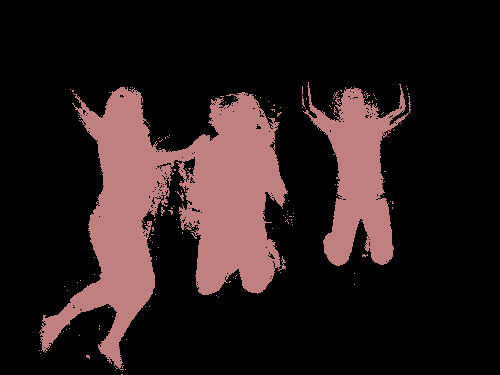
\includegraphics[height=0.123\linewidth]{fig/val_crf_vis/bbox_crf/2008_003546.png} &
    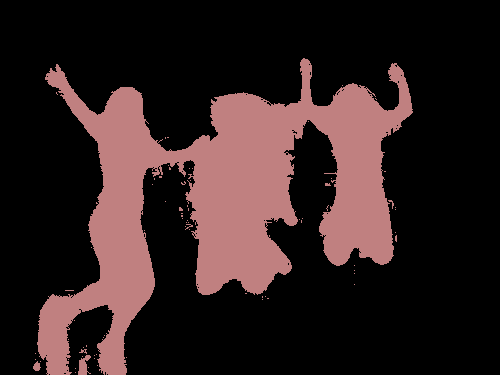
\includegraphics[height=0.123\linewidth]{fig/val_crf_vis/strongweak/2008_003546.png} &
    
\includegraphics[height=0.123\linewidth]{fig/val_crf_vis/cocomix/2008_003546.png} \\
    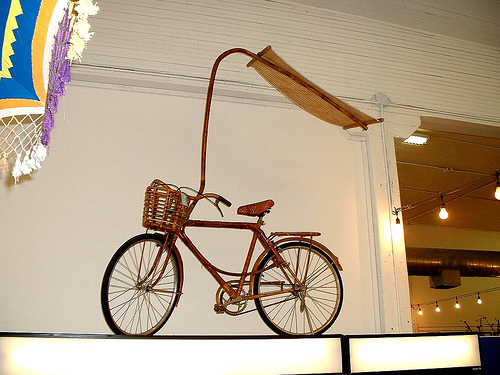
\includegraphics[height=0.123\linewidth]{fig/val_crf_vis/img/2008_004363.jpg} &
    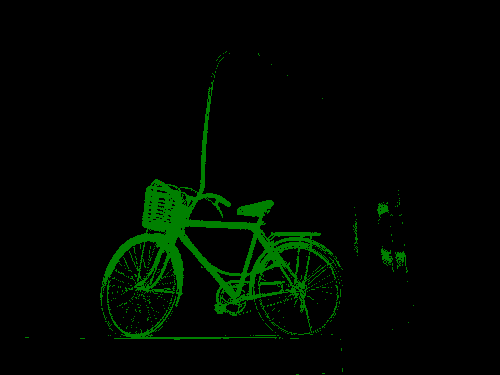
\includegraphics[height=0.123\linewidth]{fig/val_crf_vis/adaweak/2008_004363.png} &
    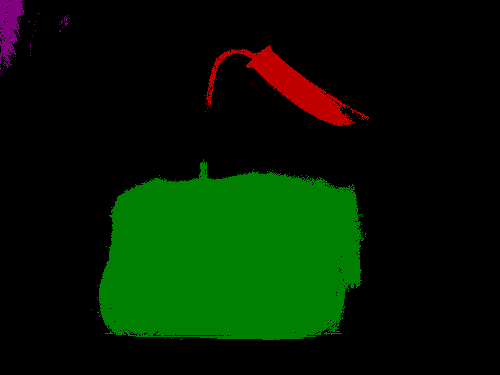
\includegraphics[height=0.123\linewidth]{fig/val_crf_vis/bbox/2008_004363.png} &
    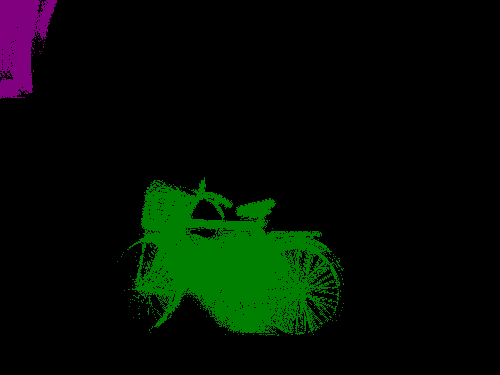
\includegraphics[height=0.123\linewidth]{fig/val_crf_vis/bbox_crf/2008_004363.png} &
    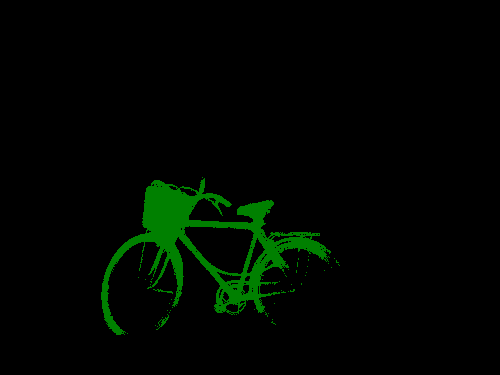
\includegraphics[height=0.123\linewidth]{fig/val_crf_vis/strongweak/2008_004363.png} &
    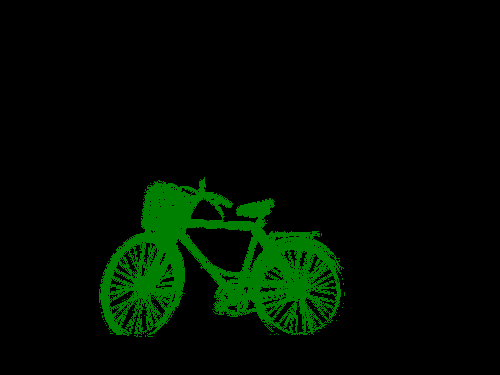
\includegraphics[height=0.123\linewidth]{fig/val_crf_vis/cocomix/2008_004363.png} \\
    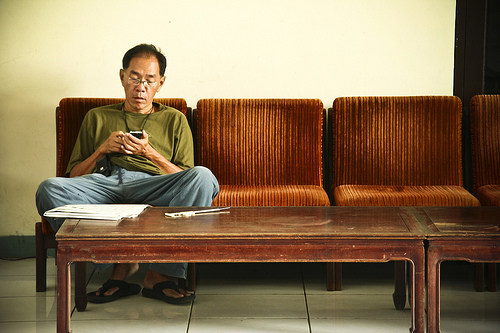
\includegraphics[height=0.11\linewidth]{fig/val_crf_vis/img/2009_001299.jpg} &
    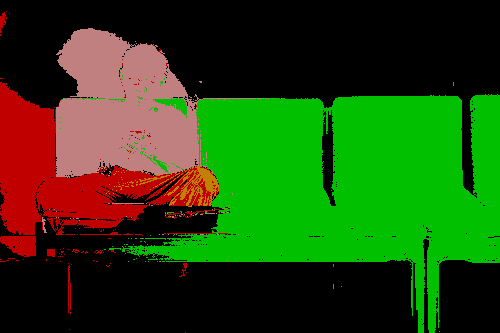
\includegraphics[height=0.11\linewidth]{fig/val_crf_vis/adaweak/2009_001299.png} &
    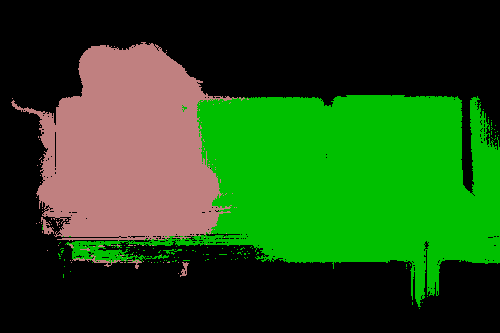
\includegraphics[height=0.11\linewidth]{fig/val_crf_vis/bbox/2009_001299.png} &
    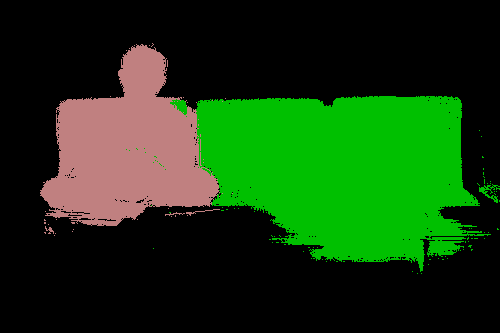
\includegraphics[height=0.11\linewidth]{fig/val_crf_vis/bbox_crf/2009_001299.png} &
    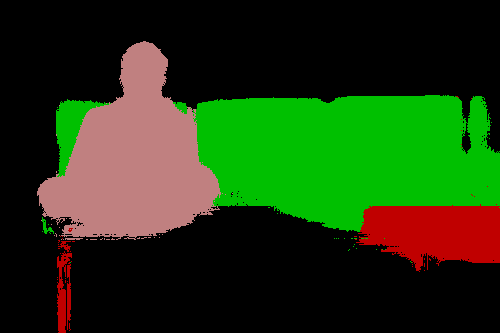
\includegraphics[height=0.11\linewidth]{fig/val_crf_vis/strongweak/2009_001299.png} &
    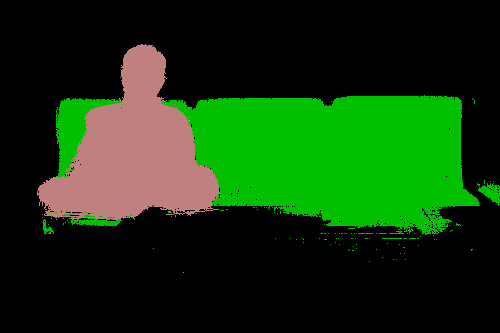
\includegraphics[height=0.11\linewidth]{fig/val_crf_vis/cocomix/2009_001299.png} \\
    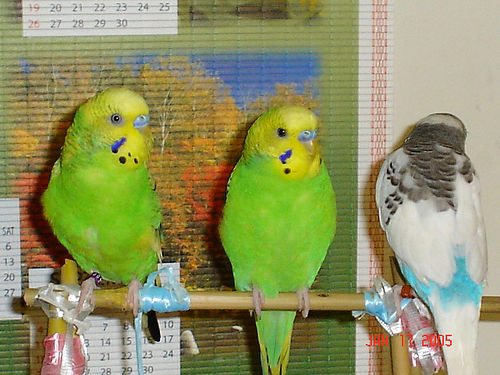
\includegraphics[height=0.123\linewidth]{fig/val_crf_vis/img/2010_004994.jpg} &
    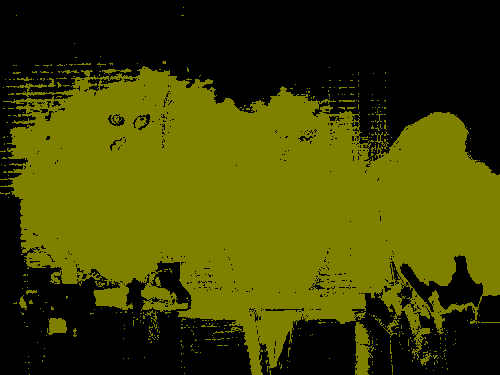
\includegraphics[height=0.123\linewidth]{fig/val_crf_vis/adaweak/2010_004994.png} &
    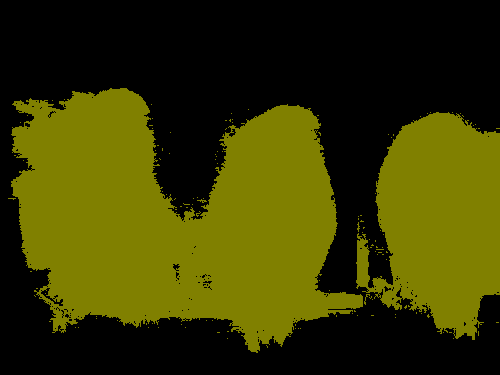
\includegraphics[height=0.123\linewidth]{fig/val_crf_vis/bbox/2010_004994.png} &
    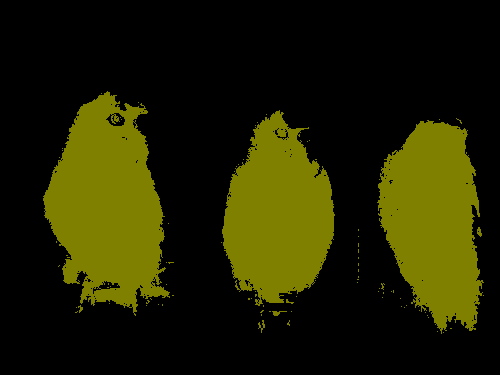
\includegraphics[height=0.123\linewidth]{fig/val_crf_vis/bbox_crf/2010_004994.png} &
    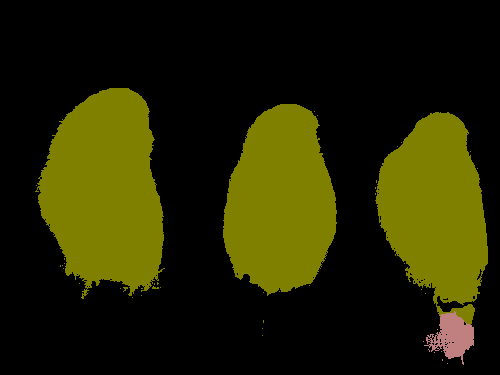
\includegraphics[height=0.123\linewidth]{fig/val_crf_vis/strongweak/2010_004994.png} &
    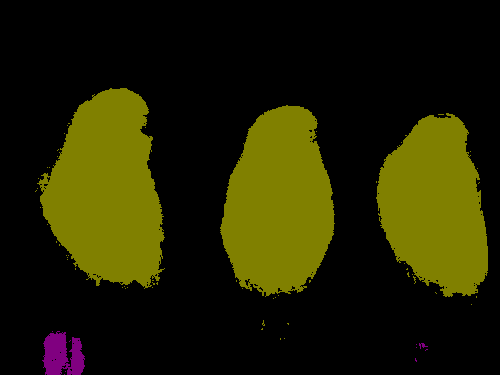
\includegraphics[height=0.123\linewidth]{fig/val_crf_vis/cocomix/2010_004994.png} \\
    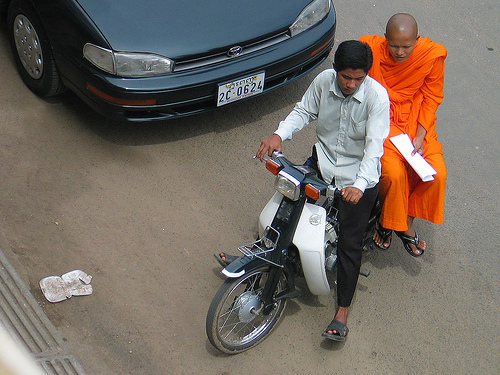
\includegraphics[height=0.122\linewidth]{fig/val_crf_vis/img/2011_002322.jpg} &
    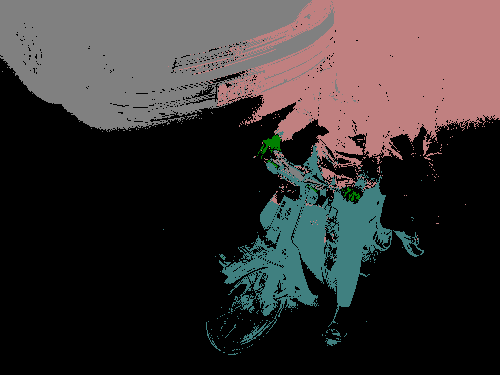
\includegraphics[height=0.122\linewidth]{fig/val_crf_vis/adaweak/2011_002322.png} &
    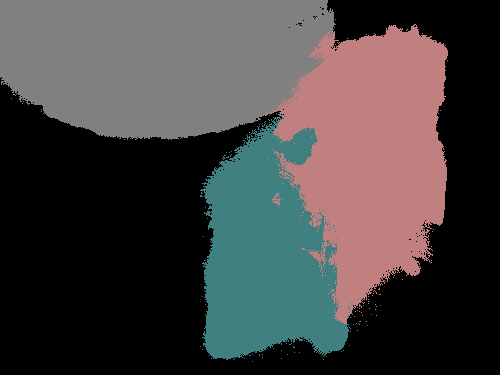
\includegraphics[height=0.122\linewidth]{fig/val_crf_vis/bbox/2011_002322.png} &
    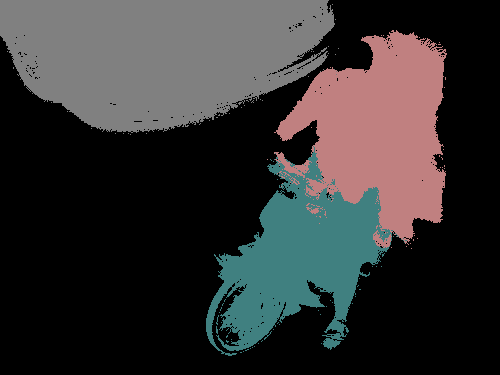
\includegraphics[height=0.122\linewidth]{fig/val_crf_vis/bbox_crf/2011_002322.png} &
    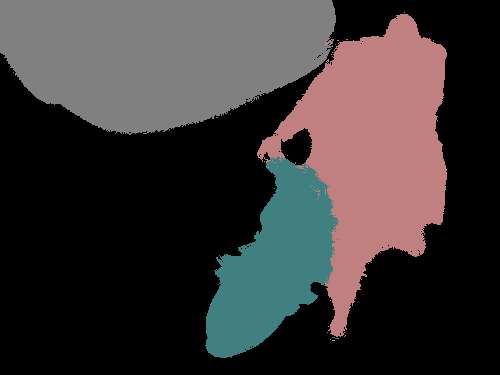
\includegraphics[height=0.122\linewidth]{fig/val_crf_vis/strongweak/2011_002322.png} &
    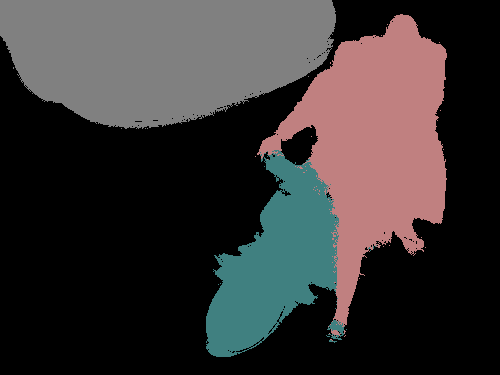
\includegraphics[height=0.122\linewidth]{fig/val_crf_vis/cocomix/2011_002322.png} \\
    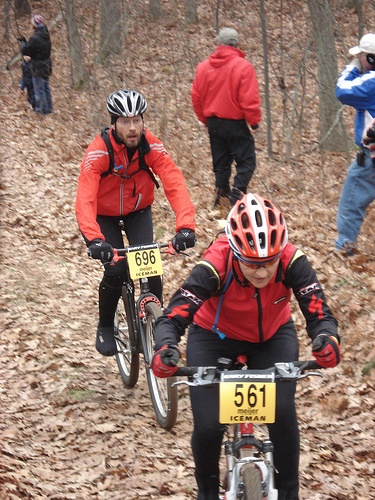
\includegraphics[height=0.13\linewidth]{fig/val_crf_vis/img/2007_001630.jpg} &
    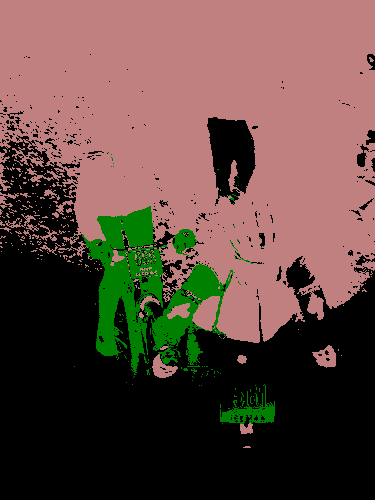
\includegraphics[height=0.13\linewidth]{fig/val_crf_vis/adaweak/2007_001630.png} &
    \includegraphics[height=0.13\linewidth]{fig/val_crf_vis/bbox/2007_001630.png} &
    \includegraphics[height=0.13\linewidth]{fig/val_crf_vis/bbox_crf/2007_001630.png} &
    \includegraphics[height=0.13\linewidth]{fig/val_crf_vis/strongweak/2007_001630.png} &
    \includegraphics[height=0.13\linewidth]{fig/val_crf_vis/cocomix/2007_001630.png} \\
    \includegraphics[height=0.15\linewidth]{fig/val_crf_vis/img/2007_005331.jpg} &
    \includegraphics[height=0.15\linewidth]{fig/val_crf_vis/adaweak/2007_005331.png} &
    \includegraphics[height=0.15\linewidth]{fig/val_crf_vis/bbox/2007_005331.png} &
    \includegraphics[height=0.15\linewidth]{fig/val_crf_vis/bbox_crf/2007_005331.png} &
    \includegraphics[height=0.15\linewidth]{fig/val_crf_vis/strongweak/2007_005331.png} &
    \includegraphics[height=0.15\linewidth]{fig/val_crf_vis/cocomix/2007_005331.png} \\
\hline \hline
    \includegraphics[height=0.11\linewidth]{fig/val_crf_vis/img/2007_000830.jpg} &
    \includegraphics[height=0.11\linewidth]{fig/val_crf_vis/adaweak/2007_000830.png} &
    \includegraphics[height=0.11\linewidth]{fig/val_crf_vis/bbox/2007_000830.png} &
    \includegraphics[height=0.11\linewidth]{fig/val_crf_vis/bbox_crf/2007_000830.png} &
    \includegraphics[height=0.11\linewidth]{fig/val_crf_vis/strongweak/2007_000830.png} &
    \includegraphics[height=0.11\linewidth]{fig/val_crf_vis/cocomix/2007_000830.png} \\
    \includegraphics[height=0.11\linewidth]{fig/val_crf_vis/img/2007_001175.jpg} &
    \includegraphics[height=0.11\linewidth]{fig/val_crf_vis/adaweak/2007_001175.png} &
    \includegraphics[height=0.11\linewidth]{fig/val_crf_vis/bbox/2007_001175.png} &
    \includegraphics[height=0.11\linewidth]{fig/val_crf_vis/bbox_crf/2007_001175.png} &
    \includegraphics[height=0.11\linewidth]{fig/val_crf_vis/strongweak/2007_001175.png} &
    \includegraphics[height=0.11\linewidth]{fig/val_crf_vis/cocomix/2007_001175.png} \\
    {\scriptsize Image} & {\scriptsize DeepLab-CRF-Adaweak} & {\scriptsize DeepLab-CRF-Bbox-Baseline} & {\scriptsize DeepLab-CRF-Bbox-DenseCRF} & {\scriptsize DeepLab-CRF-StrongWeak} & {\scriptsize DeepLab-CRF-COCO} \\
  \end{tabular}
  }
  %\vspace{-0.3cm}
  \caption{Visualization results on VOC 2012-val. For each row, we show the input image, the segmentation result delivered by adaweak, bbox, bbox-crf, strongweak, coco. The results are refined by DenseCRF. We show difficult examples in the last two rows.} 
  \label{fig:ValResults}
\end{figure*}





{\color{blue} REMEMBER to put the links (test results) in the supplementary material if main paper has no space.}
\begin{table*}[ht]\scriptsize
 \caption{Pixel IoU (\%) on the PASCAL VOC 2012 test set, using the trainval set for training.}
\setlength{\tabcolsep}{3pt}
%\hspace{-1.8cm}
\resizebox{2.1\columnwidth}{!}{
\begin{tabular}{|l||c*{20}{|c}||c|}
\hline 
Method          & bkg &  aero & bike & bird & boat & bottle& bus & car  &  cat & chair& cow  &table & dog  & horse & mbike& person& plant&sheep& sofa &train & tv   & mean \\
\hline \hline
Idiap-base+ILP+sppxl      & 74.7 & 38.8 & 19.8 & 27.5 & 21.7 & 32.8 & 40.0 & 50.1 & 47.1 & 7.2 & 44.8 & 15.8 & 49.4 & 47.3 & 36.6 & 36.4 & 24.3 & 44.5 & 21.0 & 31.5 & 41.3 & 35.8 \\
Idiap-base+ILP+seg        & 78.7 & 48.0 & 21.2 & 31.1 & 28.4 & 35.1 & 51.4 & 55.5 & 52.8 & 7.8 & 56.2 & 19.9 & 53.8 & 50.3 & 40.0 & 38.6 & 27.8 & 51.8 & 24.7 & 33.3 & 46.3 & 40.6 \\
\hline \hline
Hypercolumn-SDS & 88.9 & 68.4 & 27.2 & 68.2 & 47.6 & 61.7 & 76.9 & 72.1 & 71.1 & 24.3 & 59.3 & 44.8 & 62.7 & 59.4 & 73.5 & 70.6 & 52.1 & 63.0 & 38.1 & 60.0 & 54.1 & 59.2 \\   
MSRA-CFM        & -    & 75.7 & 26.7 & 69.5 & 48.8 & 65.6 & 81.0 & 69.2 & 73.3 & 30.0 & 68.7 & 51.5 & 69.1 & 68.1 & 71.7 & 67.5 & 50.4 & 66.5 & 44.4 & 58.9 & 53.5 & 61.8 \\
FCN-8s          & -    & 76.8 & 34.2 & 68.9 & 49.4 & 60.3 & 75.3 & 74.7 & 77.6 & 21.4 & 62.5 & 46.8 & 71.8 & 63.9 & 76.5 & 73.9 & 45.2 & 72.4 & 37.4 & 70.9 & 55.1 & 62.2 \\
TTI-Zoomout-16  & 89.8 & 81.9 & 35.1 & 78.2 & 57.4 & 56.5 & 80.5 & 74.0 & 79.8 & 22.4 & 69.6 & 53.7 & 74.0 & 76.0 & 76.6 & 68.8 & 44.3 & 70.2 & 40.2 & 68.9 & 55.3 & 64.4 \\
DeepLab-CRF     & 92.1 & 78.4 & 33.1 & 78.2 & 55.6 & 65.3 & 81.3 & 75.5 & 78.6 & 25.3 & 69.2 & 52.7 & 75.2 & 69.0 & 79.1 & 77.6 & 54.7 & 78.3 & 45.1 & 73.3 & 56.2 & 66.4 \\ 
\hline \hline
DeepLab-CRF-Adaweak & 76.4 & 37.0 & 17.6 & 38.2 & 26.6 & 37.1 & 51.9 & 43.3 & 48.1 & 16.8 & 44.6 & 27.9 & 46.5 & 46.2 & 46.6 & 30.3 & 28.9 & 42.0 & 30.0 & 43.8 & 39.3 & 39.0 \\
DeepLab-CRF-Bbox-Baseline    & 82.9 & 43.6 & 22.5 & 50.5 & 45.0 & 62.5 & 76.0 & 66.5 & 61.2 & 25.3 & 55.8 & 52.1 & 56.6 & 48.1 & 60.1 & 58.2 & 49.5 & 58.3 & 40.7 & 62.3 & 61.1 & 54.2 \\
DeepLab-CRF-Bbox-DenseCRF    & 89.9 & 69.3 & 28.2 & 71.9 & 43.4 & 59.7 & 74.3 & 69.0 & 76.7 & 23.5 & 64.6 & 47.1 & 71.0 & 64.0 & 72.8 & 72.4 & 50.4 & 72.0 & 40.2 & 63.4 & 44.5 & 60.4 \\
DeepLab-CRF-StrongWeak1(1.5K) & 91.4 & 77.3 & 38.2 & 73.9 & 47.6 & 57.9 & 80.0 & 76.4 & 74.7 & 22.8 & 70.0 & 42.0 & 70.9 & 71.9 & 79.1 & 70.7 & 47.8 & 77.1 & 36.1 & 68.1 & 59.8 & 63.5 \\
DeepLab-CRF-StrongWeak2(3K) & 92.3 & 81.3 & {\bf 43.8} & 78.3 & 50.2 & 60.4 & 81.2 & 77.5 & 77.5 & 26.8 & 70.8 & 47.0 & 74.8 & 73.0 & 80.8 & 76.0 & 50.8 & 78.0 & 39.7 & 72.9 & 60.9 & 66.4 \\
DeepLabe-CRF-COCO & {\bf 93.2} & {\bf 85.3} & 36.2 & {\bf 84.8} & {\bf 61.2} & {\bf 67.5} & {\bf 84.7} & {\bf 81.4} & {\bf 81.0} & {\bf 30.8} & {\bf 73.8} & {\bf 53.8} & {\bf 77.5} & {\bf 76.5} & {\bf 82.3} & {\bf 81.6} & {\bf 56.3} & {\bf 78.9} & {\bf 52.3} & {\bf 76.6} & {\bf 63.3} & {\bf 70.4} \\
\hline
 \end{tabular}
} \label{tab:voc2012}
\end{table*}

 %%% Local Variables:
 %%% mode: latex
 %%% TeX-master: "top.tex"
 %%% End:
